\chapter{Bias-varianza ed ensemble}\label{ch-15}

La SLT ha spiegato underfitting e overfitting tramite la complessità del
modello e il numero di dati. La \textbf{decomposizione bias-varianza}
offre un altro punto di vista, complementare: considera il fatto che il
training set è \textbf{una sola} delle possibili realizzazioni dei dati,
e scompone l'errore atteso in tre componenti --- \textbf{bias},
\textbf{varianza} e \textbf{rumore}. Da qui si arriva in modo naturale
agli \textbf{ensemble} (bagging, boosting), che sfruttano proprio la
riduzione della varianza.

\section{L'idea}\label{lidea}

Un training set è solo una possibile realizzazione dall'universo dei
dati: \textbf{training set diversi producono stime diverse}. L'errore
atteso (sui vari training set) in un punto \(\mathbf{x}\) si scompone
in:

\begin{itemize}
\tightlist
\item
  \textbf{Bias}: quantifica la discrepanza tra la funzione vera e
  \(h(\mathbf{x})\) (mediata sui dati). È alto se \(H\) è troppo piccolo
  (modello troppo rigido).
\item
  \textbf{Varianza}: quantifica la variabilità della risposta del
  modello \(h\) per diverse realizzazioni dei dati di training. È dovuta
  a un'eccessiva flessibilità.
\item
  \textbf{Rumore}: le etichette contengono un errore casuale (ad
  esempio, per un dato \(\mathbf{x}\) ci possono essere più valori di
  \(d\) possibili).
\end{itemize}

Si assume lo scenario della \textbf{regressione} con target \(y\) e loss
quadratica.

\section{Analisi nella regressione}\label{analisi-nella-regressione}

Supponiamo esempi \(\langle \mathbf{x}, y\rangle\) con funzione vera
\(y = f(\mathbf{x}) + \varepsilon\), dove \(\varepsilon\) è rumore
gaussiano con media zero e deviazione standard \(\sigma\). Con la
regressione lineare, dato un insieme di esempi
\(\langle\mathbf{x}_i, y_i\rangle\), \(i = 1..l\), si adatta un'ipotesi
lineare \(h(\mathbf{x}) = \mathbf{w}\mathbf{x} + w_0\) minimizzando
\(\sum_{i=1}^l (y_i - h(\mathbf{x}_i))^2\). Due fatti:

\begin{enumerate}
\def\labelenumi{\arabic{enumi}.}
\tightlist
\item
  per la classe di ipotesi scelta (lineari), per alcune \(f\) si avrà un
  \textbf{errore di predizione sistematico};
\item
  a seconda del dataset, i parametri \(\mathbf{w}\) trovati
  \textbf{saranno diversi}.
\end{enumerate}

\begin{boxexample}{20 punti e 50 fit}

Funzione vera \(y = x + 2\sin(1{,}5x) + \mathcal{N}(0; 0{,}2)\). Con 20
punti si adatta una retta. Ripetendo con 50 dataset diversi (ciascuno di
20 punti), si ottengono 50 rette diverse.

\end{boxexample}

\begin{figure}[htbp]
\centering
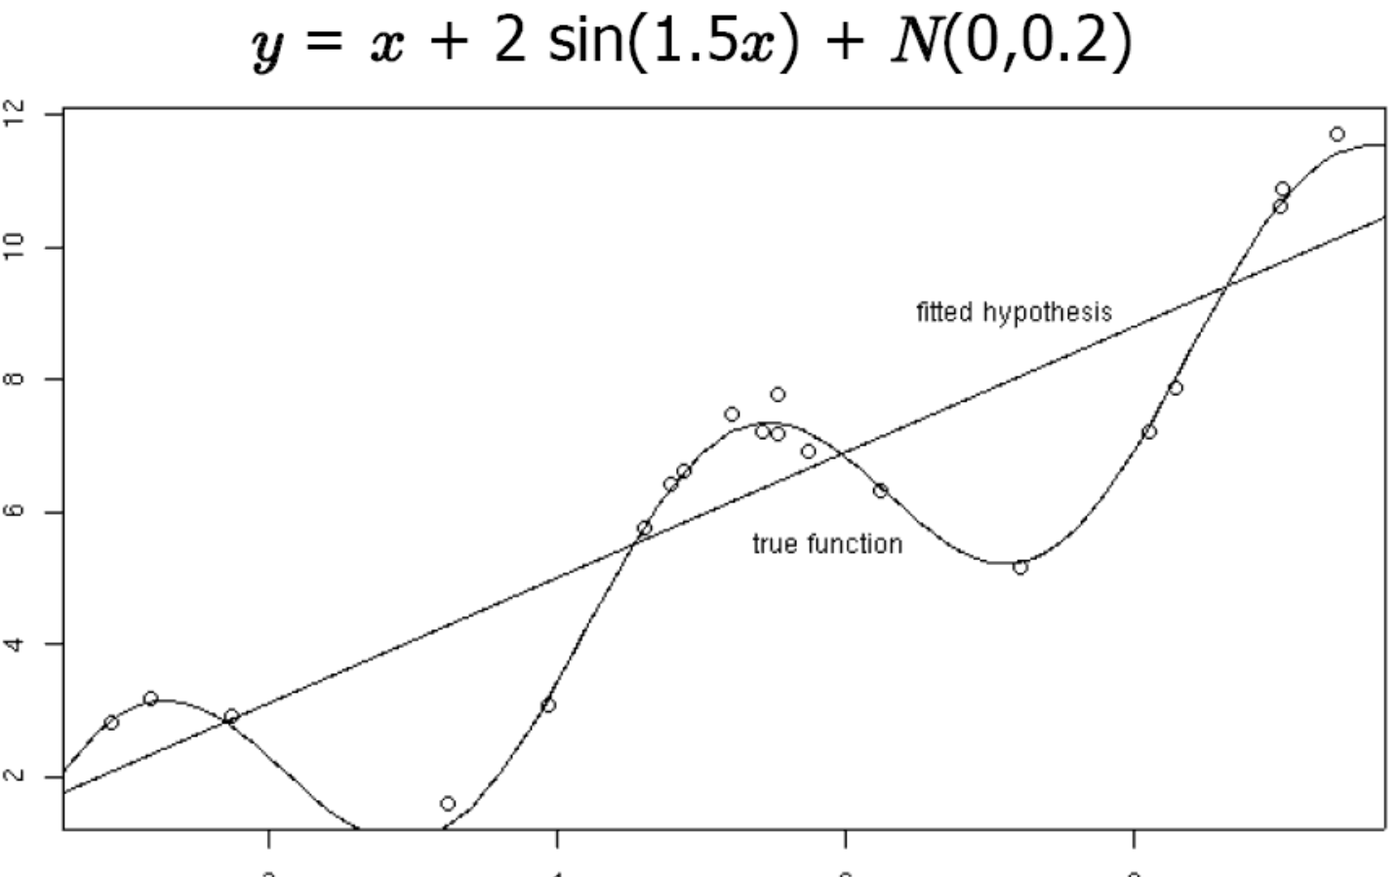
\includegraphics[width=0.63\linewidth,height=0.42\textheight,keepaspectratio]{images/15-bv_20punti.png}
\caption{Un dataset di 20 punti, la funzione vera e l'ipotesi lineare adattata.}
\end{figure}

\begin{figure}[htbp]
\centering
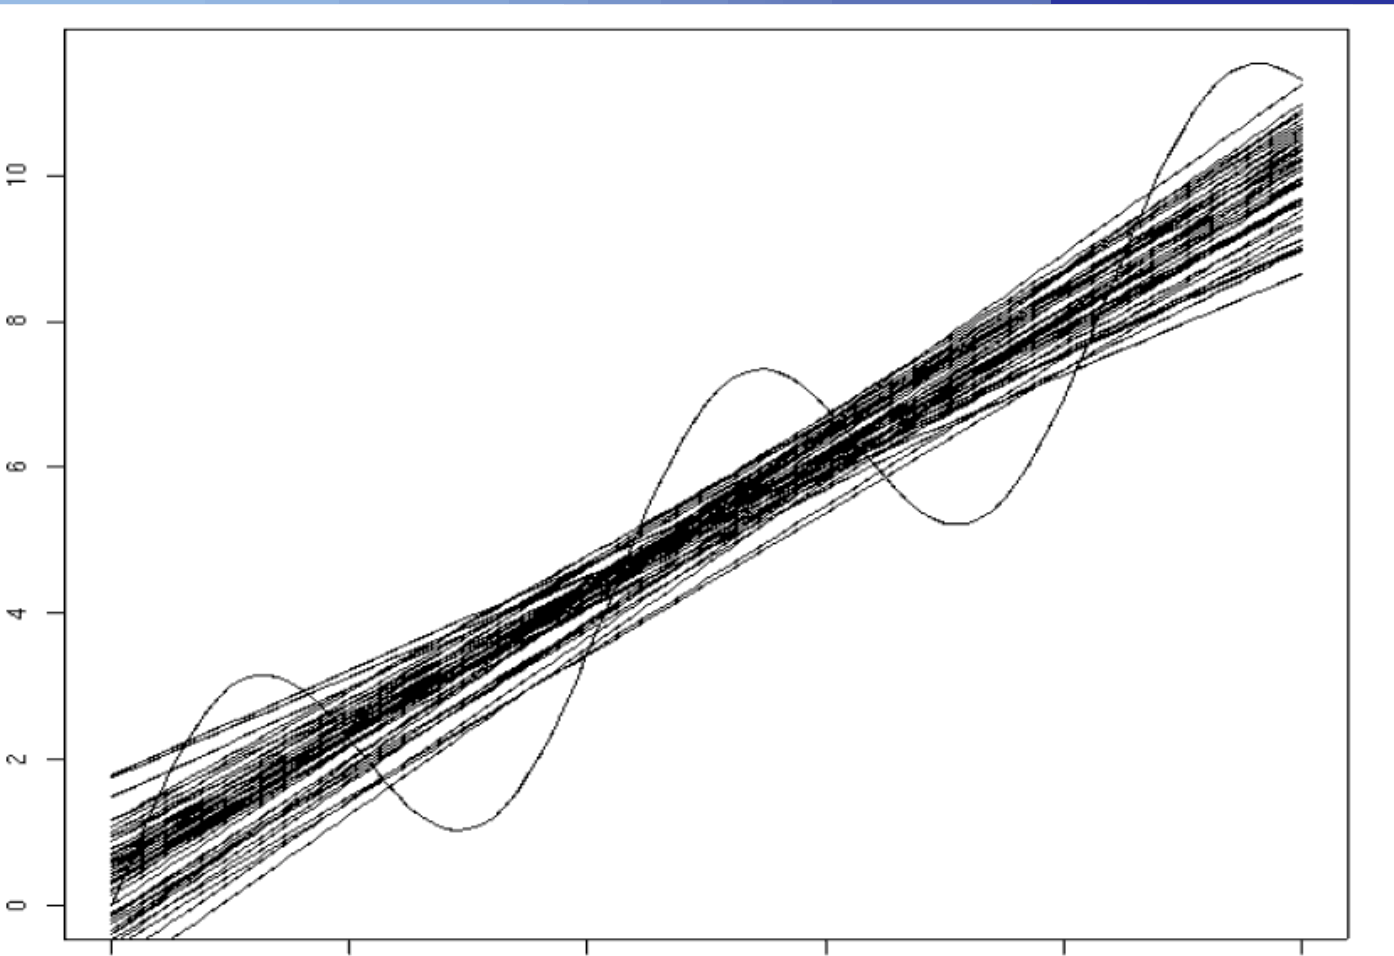
\includegraphics[width=0.63\linewidth,height=0.42\textheight,keepaspectratio]{images/15-bv_50fit.png}
\caption{50 fit, ciascuno su 20 punti: le rette variano da un dataset all'altro.}
\end{figure}

\subsection{L'errore di predizione
atteso}\label{lerrore-di-predizione-atteso}

Dato un nuovo punto \(\mathbf{x}\), qual è l'\textbf{errore di
predizione atteso}? Si assume che i dati siano estratti in modo
\textbf{i.i.d.} (indipendenti e identicamente distribuiti) da un'unica
distribuzione \(P\). L'obiettivo è calcolare, per un \(\mathbf{x}\)
arbitrario, \[
E_P\big[(y - h(\mathbf{x}))^2\big],
\] dove \(y\) è il valore di \(\mathbf{x}\) che potrebbe comparire in un
dataset, e l'aspettativa è \textbf{su tutti i training set} estratti
secondo \(P\). Attenzione: per ogni training set ``estratto'' c'è una
\(h\) diversa (e un \(y\) diverso).

\subsection{Richiamo di statistica}\label{richiamo-di-statistica}

Per una variabile aleatoria discreta \(Z\):
\(\bar Z = E_P[Z] = \sum_i z_i P(z_i)\) e
\(\operatorname{Var}[Z] = E[(Z - \bar Z)^2]\).

\begin{boxtheorem}{Lemma della varianza}

\[
\operatorname{Var}[Z] = E[Z^2] - \bar Z^2 \qquad\Longleftrightarrow\qquad E[Z^2] = \bar Z^2 + \operatorname{Var}[Z].
\] \textbf{Dimostrazione.}
\(\operatorname{Var}[Z] = \sum_i (z_i - \bar Z)^2 P(z_i) = \sum_i z_i^2P(z_i) - 2\bar Z\sum_i z_iP(z_i) + \bar Z^2\sum_i P(z_i) = E[Z^2] - 2\bar Z^2 + \bar Z^2 = E[Z^2] - \bar Z^2\).

\end{boxtheorem}

\subsection{La decomposizione}\label{la-decomposizione}

Sviluppando il quadrato e usando la linearità dell'aspettativa (e il
fatto che \(y\) e \(h(\mathbf{x})\) sono indipendenti, perché \(y\) è un
nuovo dato e \(h\) dipende dal training set): \[
E_P\big[(y - h(\mathbf{x}))^2\big] = E_P\big[h(\mathbf{x})^2 - 2yh(\mathbf{x}) + y^2\big] = E_P\big[h(\mathbf{x})^2\big] + E_P\big[y^2\big] - 2E_P[y]\,E_P[h(\mathbf{x})].
\]

Sia \(\bar h(\mathbf{x}) = E_P[h(\mathbf{x})]\) la \textbf{predizione
media} dell'ipotesi in \(\mathbf{x}\), quando \(h\) è addestrata su dati
estratti da \(P\).

\begin{itemize}
\tightlist
\item
  \textbf{Primo termine}, con il lemma:
  \(E_P[h(\mathbf{x})^2] = E_P\big[(h(\mathbf{x}) - \bar h(\mathbf{x}))^2\big] + \bar h(\mathbf{x})^2\).
\item
  Si noti che
  \(E_P[y] = E_P[f(\mathbf{x}) + \varepsilon] = f(\mathbf{x})\) (il
  rumore ha media zero).
\item
  \textbf{Secondo termine}, con il lemma:
  \(E_P[y^2] = E_P\big[(y - f(\mathbf{x}))^2\big] + f(\mathbf{x})^2\).
\end{itemize}

Mettendo tutto insieme: \[
\begin{aligned}
E_P\big[(y - h(\mathbf{x}))^2\big] &= E_P\big[(h(\mathbf{x}) - \bar h(\mathbf{x}))^2\big] + \underbrace{\bar h(\mathbf{x})^2 - 2f(\mathbf{x})\bar h(\mathbf{x}) + f(\mathbf{x})^2}_{(\bar h(\mathbf{x}) - f(\mathbf{x}))^2} + E_P\big[(y - f(\mathbf{x}))^2\big] \\
&= \underbrace{E_P\big[(h(\mathbf{x}) - \bar h(\mathbf{x}))^2\big]}_{\text{varianza}} + \underbrace{\big(\bar h(\mathbf{x}) - f(\mathbf{x})\big)^2}_{\text{bias}^2} + \underbrace{E_P\big[(y - f(\mathbf{x}))^2\big]}_{\text{rumore}^2} \\
&= \operatorname{Var}[h(\mathbf{x})] + \operatorname{Bias}[h(\mathbf{x})]^2 + E_P[\varepsilon^2] = \operatorname{Var}[h(\mathbf{x})] + \operatorname{Bias}[h(\mathbf{x})]^2 + \sigma^2.
\end{aligned}
\]

\begin{boxtheorem}{Decomposizione bias-varianza}

\[
\text{Errore di predizione atteso} = \text{Varianza} + \text{Bias}^2 + \text{Rumore}^2.
\]

\end{boxtheorem}

\subsection{Interpretazione delle tre
componenti}\label{interpretazione-delle-tre-componenti}

\begin{itemize}
\tightlist
\item
  \textbf{Bias} \(\big(\bar h(\mathbf{x}) - f(\mathbf{x})\big)^2\): la
  discrepanza tra la funzione vera e la predizione \textbf{media} sui
  diversi training set. È un \textbf{errore sistematico}, dovuto ad
  esempio a uno spazio \(H\) troppo piccolo o a un modello troppo
  rigido.
\item
  \textbf{Varianza}: la variabilità della risposta del modello per
  diverse realizzazioni del training set. È dovuta a una
  \textbf{flessibilità eccessiva}.
\item
  \textbf{Rumore}: anche la soluzione ottima può sbagliare (ad esempio
  se per un dato \(\mathbf{x}\) sono possibili più valori di \(d\)). È
  \textbf{irriducibile}: non dipende dal modello e rappresenta una
  tolleranza sulla risposta (\(\sigma\)).
\end{itemize}

\begin{figure}[htbp]
\centering
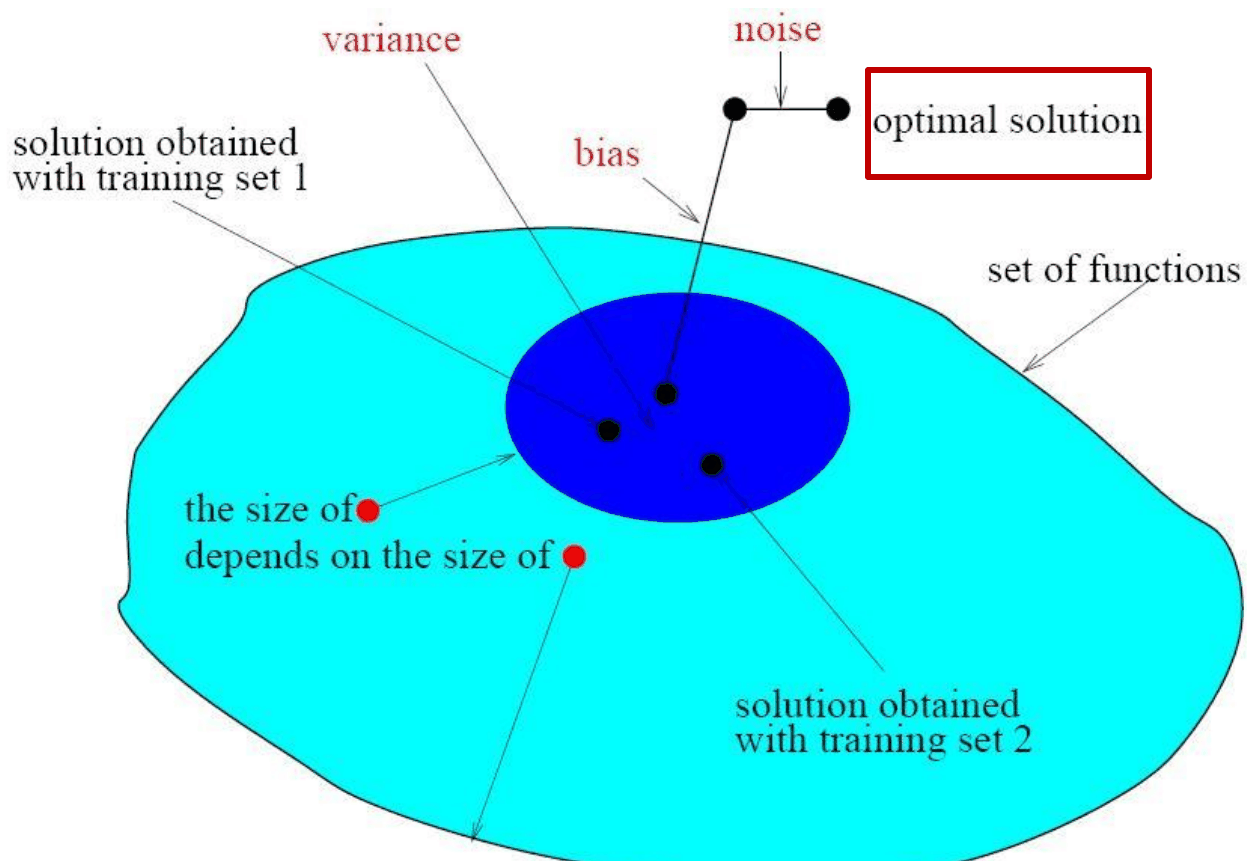
\includegraphics[width=0.66\linewidth,height=0.42\textheight,keepaspectratio]{images/15-bv_vista-grafica.png}
\caption{Vista grafica: training set diversi producono soluzioni diverse
(varianza); la loro media dista dall'ottimo (bias); l'ottimo stesso
dista dai dati per il rumore.}
\end{figure}

Tornando all'esempio: il \textbf{bias} è evidente nella media \(\bar h\)
delle 50 rette, che resta lontana dalla funzione vera ondulata (il
modello lineare è troppo rigido); la \textbf{varianza} è la dispersione
delle 50 rette attorno a \(\bar h\); il \textbf{rumore} è la dispersione
dei dati attorno alla funzione vera.

\begin{figure}[htbp]
\centering
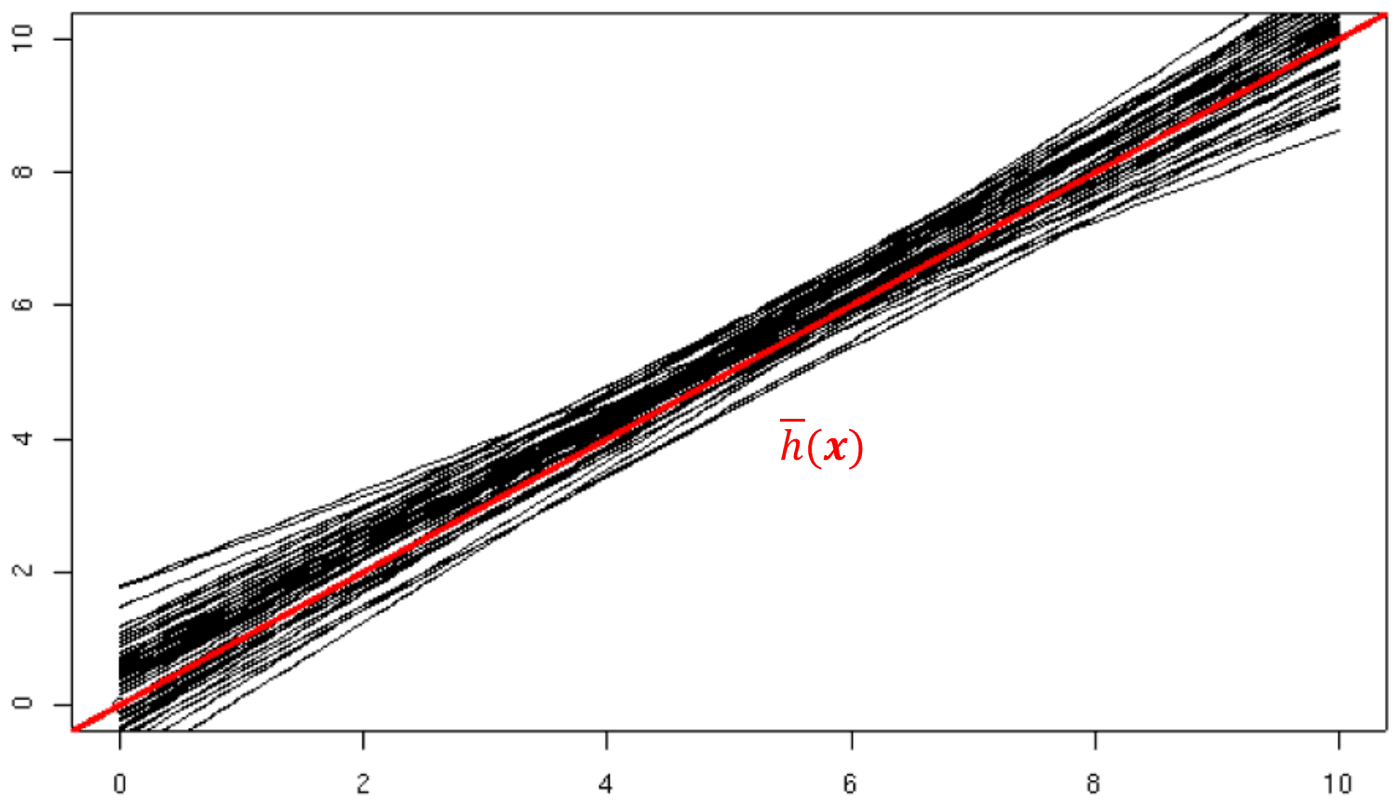
\includegraphics[width=0.63\linewidth,height=0.42\textheight,keepaspectratio]{images/15-bv_varianza.png}
\caption{La varianza: la dispersione delle ipotesi attorno alla predizione media
\(\bar h(\mathbf{x})\) (in rosso).}
\end{figure}

\begin{boxexample}{L'analogia delle freccette}

\begin{center}
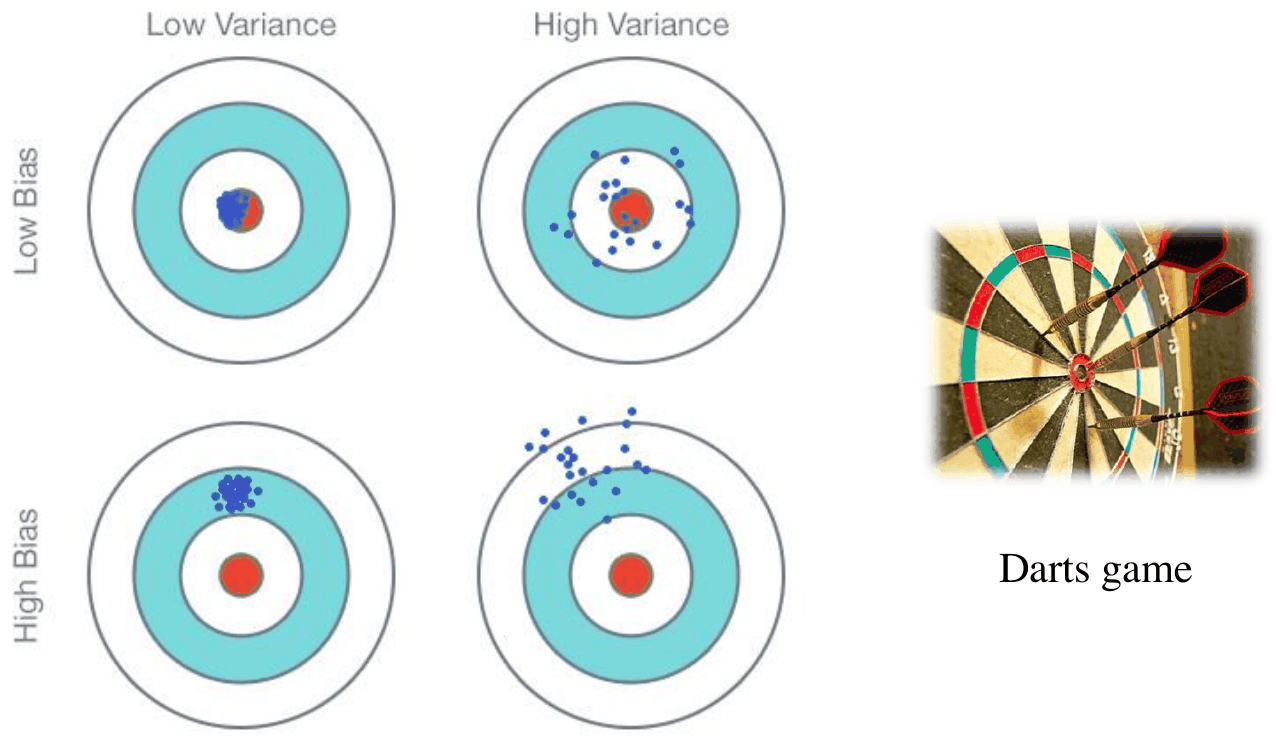
\includegraphics[width=0.63\linewidth,height=0.42\textheight,keepaspectratio]{images/15-bv_freccette.png}
\end{center}

Il centro è la funzione vera, ogni freccetta è un modello addestrato su
un training set diverso. \textbf{Alto bias e bassa varianza} (in basso a
sinistra) corrisponde all'\textbf{underfitting}; \textbf{basso bias e
alta varianza} (in alto a destra) all'\textbf{overfitting}. L'analogia
non è perfetta per il ML, ma aiuta.

\end{boxexample}

\section{Bias, varianza e
regolarizzazione}\label{bias-varianza-e-regolarizzazione}

Ricordiamo la loss regolarizzata: \[
\text{Loss}(\mathbf{w}) = \underbrace{\sum_p\big(d_p - o(\mathbf{x}_p)\big)^2}_{\text{termine sui dati}} + \underbrace{\lambda\|\mathbf{w}\|^2}_{\text{penalità}}.
\] Variando \(\lambda\) si ottengono soluzioni meno regolarizzate
(complesse, \(\lambda\) basso) o più regolarizzate (meno complesse,
\(\lambda\) alto). (L'intercetta è tipicamente esclusa dalla penalità.)

Esempio di Bishop: 25 dataset estratti dalla sinusoide, modello (una
rete RBF) addestrato su ciascuno con diversi valori di \(\lambda\).

\begin{figure}[htbp]
\centering
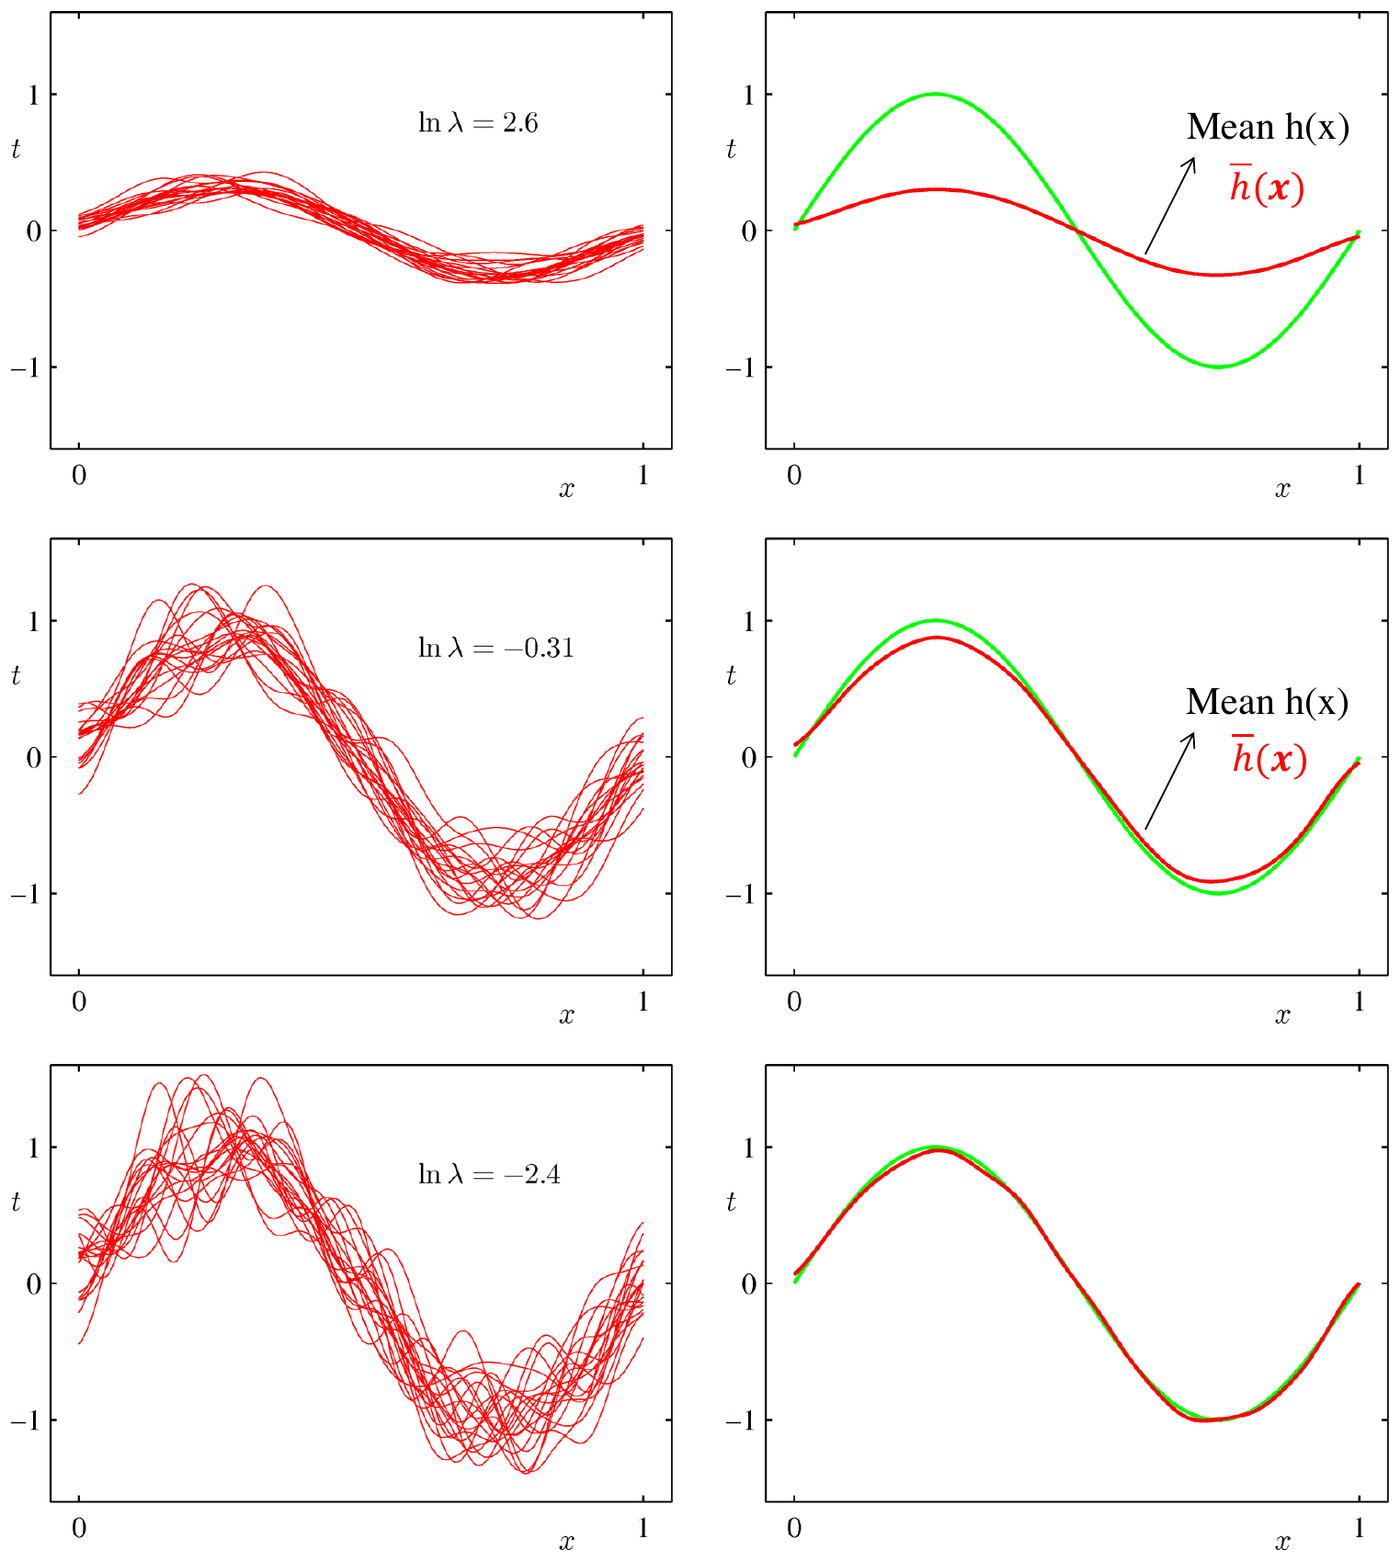
\includegraphics[width=0.80\linewidth,height=0.42\textheight,keepaspectratio]{images/15-bv_lambda.png}
\caption{Effetto di \(\lambda\) su bias e varianza: \(\ln\lambda = 2{,}6\) (in
alto), \(-0{,}31\) (al centro), \(-2{,}4\) (in basso). A sinistra le 25
ipotesi, a destra la loro media \(\bar h(x)\) (rossa) e la funzione vera
(verde).}
\end{figure}

\begin{itemize}
\tightlist
\item
  \textbf{\(\lambda\) alto}: \textbf{alto bias, bassa varianza}. La
  penalità domina, il modello dipende poco dai dati ed è ``troppo
  rigido'': le curve si somigliano ma la loro media è lontana dalla
  sinusoide.
\item
  \textbf{\(\lambda\) medio}: bias più basso, varianza più alta.
  Diminuendo \(\lambda\) si dipende di più dal particolare training set.
\item
  \textbf{\(\lambda\) molto basso}: \textbf{basso bias, alta varianza}.
  L'errore di test per un singolo training set può essere alto (per la
  componente di varianza), ma anche se le curve sono molto diverse tra
  loro, \textbf{in media} sono corrette (grafico a destra).
\end{itemize}

\begin{figure}[htbp]
\centering
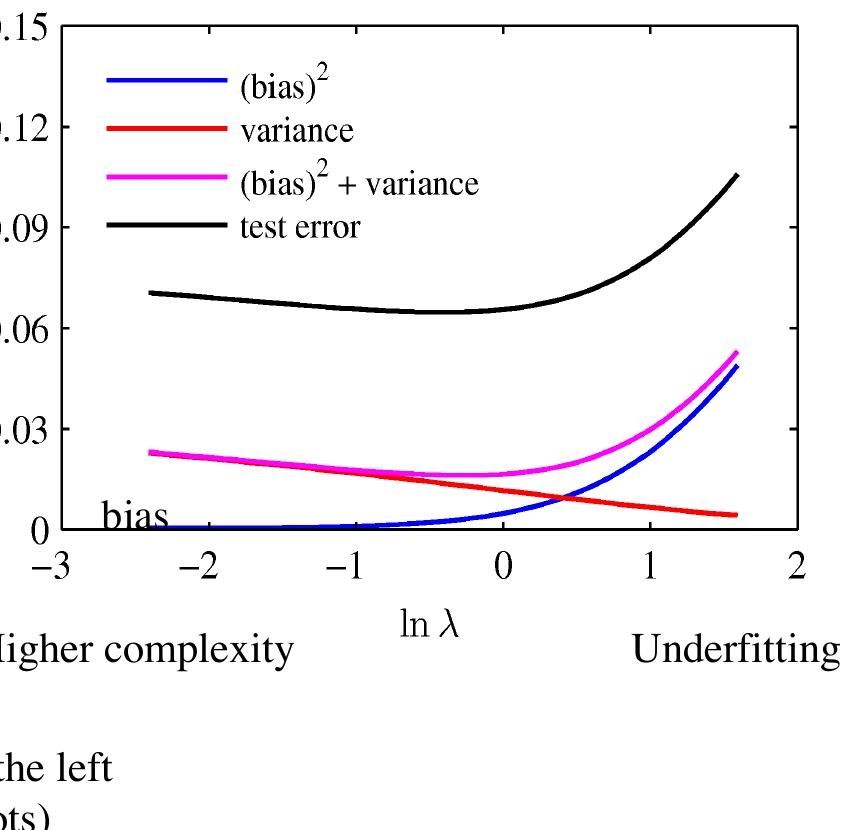
\includegraphics[width=0.51\linewidth,height=0.42\textheight,keepaspectratio]{images/15-bv_tradeoff.png}
\caption{Il compromesso bias-varianza al variare di \(\ln\lambda\). Attenzione:
qui la complessità è più alta a \textbf{sinistra} (al contrario dei
grafici usuali).}
\end{figure}

Un modello \textbf{sovra-regolarizzato} (grande \(\lambda\)) ha bias
alto; uno \textbf{sotto-regolarizzato} (piccolo \(\lambda\)) ha varianza
alta. Di nuovo, \textbf{il compromesso}: il minimo di bias² + varianza
coincide circa con il minimo dell'errore di test.

La stessa figura vista nella validazione
(\href{09\%20-\%20Validazione\%20(parte\%201)\%20-\%20model\%20selection\%20e\%20assessment}{09
- Validazione (parte 1) - model selection e assessment}) mostra, al
crescere della complessità, errori di training e test su 100 training
set: un modello complesso ha \textbf{bias basso e varianza alta}, quindi
rischio di overfitting, e a seconda del training set si può essere
fortunati o sfortunati.

\begin{boxtip}{Il collegamento con la SLT}

Bias e varianza sono un'altra faccia del compromesso tra adattamento ai
dati e complessità: il bias corrisponde all'incapacità del modello di
rappresentare la funzione (alto \(R_{emp}\), underfitting), la varianza
alla sensibilità ai dati specifici (alta VC-confidence, overfitting).

\end{boxtip}

\section{Ensemble learning}\label{ensemble-learning}

L'idea degli \textbf{ensemble} è sfruttare \textbf{più modelli}
combinandone le risposte.

Nel caso più semplice (\textbf{schema a voto}):

\begin{itemize}
\tightlist
\item
  \textbf{Regressione}: comitato a media semplice,
  \(o(\mathbf{x}) = \frac{1}{K}\sum_{i=1}^K h_i(\mathbf{x})\).
\item
  \textbf{Classificazione}: voto su molti classificatori (purché diano
  risposte \textbf{diversificate}), oppure si classifica dopo aver
  mediato le uscite continue.
\end{itemize}

In alternativa (\textbf{stacking}) il combinatore è a sua volta un
modello di ML.

\begin{boxtheorem}{Il comitato non è peggiore della media dei suoi membri}

Per una loss convessa come l'errore quadratico, l'errore del comitato è
minore o uguale alla media degli errori dei singoli modelli: \[
\text{loss}\big(E_i[h_i]\big) \le E_i\big[\text{loss}(h_i)\big].
\] (È la disuguaglianza di Jensen.) Esempio con target \(t = 5\) e due
modelli che predicono 2 e 4: la media degli errori è
\(\frac{(5-2)^2 + (5-4)^2}{2} = 5\), mentre l'errore del comitato
(\(o = 3\)) è \((5-3)^2 = 4\). Con predizioni 6 e 4: media degli errori
\(\frac{1 + 1}{2} = 1\), errore del comitato \((5-5)^2 = 0\).

\end{boxtheorem}

\subsection{Bagging (bootstrap
aggregating)}\label{bagging-bootstrap-aggregating}

\begin{itemize}
\tightlist
\item
  Si addestrano \(K\) classificatori su \textbf{sottoinsiemi diversi}
  del training set, differenziati con il \textbf{bootstrap}
  (ricampionamento con reinserimento).
\item
  Regressione: si usa la media; classificazione: voto dei \(K\)
  classificatori.
\end{itemize}

Il legame con bias-varianza è diretto (si ricordi il caso ``\(\lambda\)
basso''): modelli ad \textbf{alta varianza} e \textbf{basso bias}
possono funzionare bene \textbf{in media}. In altri termini, \textbf{la
media delle \(h\) riduce la varianza} senza aumentare il bias. Inoltre
il bagging tende ad aumentare il \textbf{margine} di un classificatore:
la media di \(K\) curve di separazione tende a stare ``nel mezzo''
(\emph{in medio stat virtus}).

\subsection{Boosting (es. AdaBoost)}\label{boosting-es.-adaboost}

Se i modelli commettono gli \textbf{stessi errori}, combinarli non
serve. Il boosting li differenzia di proposito:

\begin{enumerate}
\def\labelenumi{\arabic{enumi}.}
\tightlist
\item
  addestra i classificatori in sequenza concentrandosi sugli
  \textbf{errori}: il secondo dà più peso alle istanze sbagliate dal
  primo (ad esempio sono più probabili nel suo training set), e così
  via;
\item
  combina i risultati con un \textbf{voto pesato}, dando più peso ai
  classificatori con errore più basso.
\end{enumerate}

Se non lo si ferma, il boosting impara a classificare correttamente
\textbf{tutte} le istanze di training usando \textbf{weak learner}
(classificatori appena migliori del caso, con errore \(< 1/2\) nel
binario), costruendo in modo incrementale modelli complessi. Può
migliorare molto le prestazioni di learner deboli; riduce il bias senza
aumentare la varianza (resiste all'overfitting) e, come il bagging,
tende a produrre curve di separazione ``nel mezzo'' (margine massimo).
Però \textbf{soffre con dati rumorosi} (che vengono pesati sempre di
più), e non risolve di per sé il problema underfitting/overfitting.

\section{Feature selection (cenni)}\label{feature-selection-cenni}

Trovare il sottoinsieme delle feature più informative per il problema
porta grandi benefici: \textbf{riduzione della dimensionalità} (effetti
sulla VC-dim delle reti, sulla curse of dimensionality\ldots),
filtraggio di informazione irrilevante e rumore (con possibili forti
miglioramenti delle prestazioni), \textbf{interpretabilità} (trovare
descrittori utili). Ma:

\begin{itemize}
\tightlist
\item
  è \textbf{computazionalmente difficile} (numero enorme di sottoinsiemi
  possibili, e ogni valutazione richiede di riaddestrare);
\item
  si usa tipicamente una \textbf{ricerca euristica} (greedy, algoritmi
  genetici o altre tecniche di ottimizzazione), includendo o meno il
  learner;
\item
  i risultati sono particolarmente sensibili al metodo di validazione:
  attenzione al \textbf{feature subset selection bias}, cioè all'errore
  di fare la selezione sull'intero dataset (vedi le slide sulla
  cross-validation).
\end{itemize}

Altri argomenti collegati: PAC learning; confronto tra principi
induttivi (SRM, MDL, inferenza bayesiana, regolarizzazione) rispetto al
controllo della complessità.

\begin{boxabstract}{Sintesi}

L'errore atteso (sui training set) si scompone in \textbf{varianza +
bias² + rumore}. Modelli rigidi (o molto regolarizzati) hanno alto bias
e bassa varianza (underfitting); modelli flessibili (poco regolarizzati)
basso bias e alta varianza (overfitting); il rumore è irriducibile. Gli
\textbf{ensemble} sfruttano la decomposizione: il \textbf{bagging} media
modelli ad alta varianza riducendola; il \textbf{boosting} combina
learner deboli concentrandosi sugli errori.

\end{boxabstract}

\begin{boxquestion}{Possibili domande d'esame}

\begin{itemize}
\tightlist
\item
  Derivare la decomposizione bias-varianza per la loss quadratica.
\item
  Cosa rappresentano bias, varianza e rumore? Quale componente è
  irriducibile?
\item
  Come variano bias e varianza con il parametro di regolarizzazione
  \(\lambda\)?
\item
  Perché un comitato non è peggiore della media dei suoi membri?
\item
  Differenza tra bagging e boosting; perché il bagging riduce la
  varianza?
\end{itemize}

\end{boxquestion}
